\documentclass[portrait,final,a0paper,fontscale=0.277]{baposter}
 \usepackage[latin1]{inputenc}
 \usepackage[T1]{fontenc}
 \usepackage[spanish]{babel}
 \usepackage{graphicx}
 
\definecolor{bgcolor2}{RGB}{100,100,120}
\definecolor{bgcolor1}{RGB}{250,250,255}
\definecolor{headercol1}{RGB}{225,225,250}
\definecolor{headercol2}{RGB}{20,20,70}
\definecolor{boxcol}{RGB}{200,200,200}



\begin{document}
\begin{poster}
	% Poster Options
	{
		bgColorOne=bgcolor1,
		bgColorTwo=bgcolor2,
		background=shadetb,
		headerColorOne=headercol1,
		headerColorTwo=headercol2,
		headershape=rounded,
		textborder=none,
		boxColorOne=headercol1,	
	}

	% Title
	{Construcci�n de un cohete de agua}
	% Authors
	{
		Eros Camacho Ruiz
	}

	 \headerbox{IM�GENES}{name=imagen,column=0,row=0}{
	 	\begin{center}
	 	\vspace{1cm}	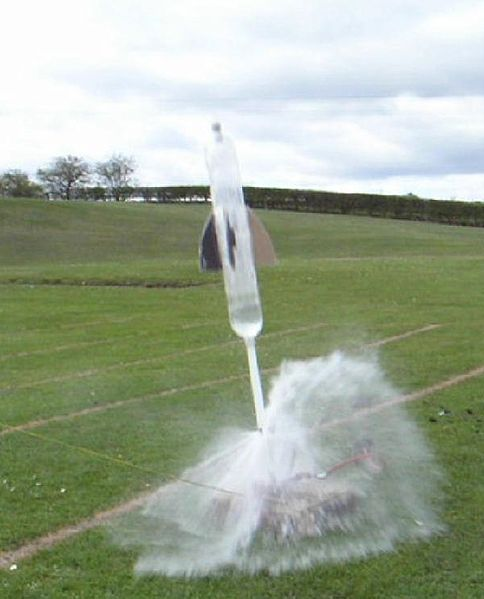
\includegraphics[width=5cm]{cohete}
	 	\end{center}
	 	\begin{center}
	 	\vspace{1cm}	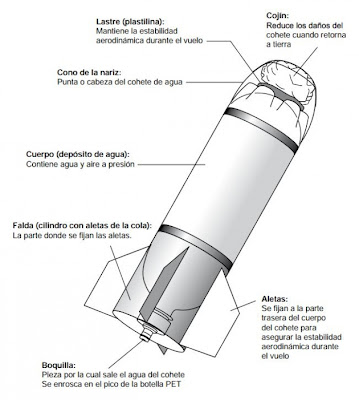
\includegraphics[width=5cm]{cohete2}
	 	\end{center}
	 	\begin{center}
	 	\vspace{1cm}	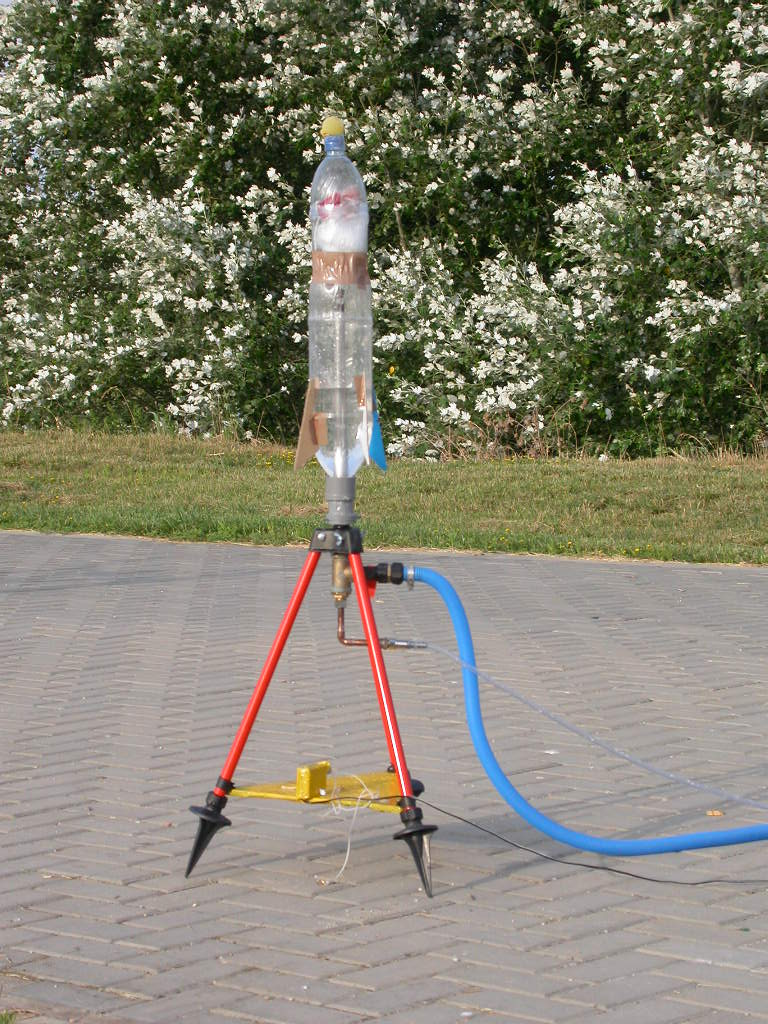
\includegraphics[width=5cm]{cohete3}
	 	\end{center}
	 	\begin{center}
	 	\vspace{1cm}	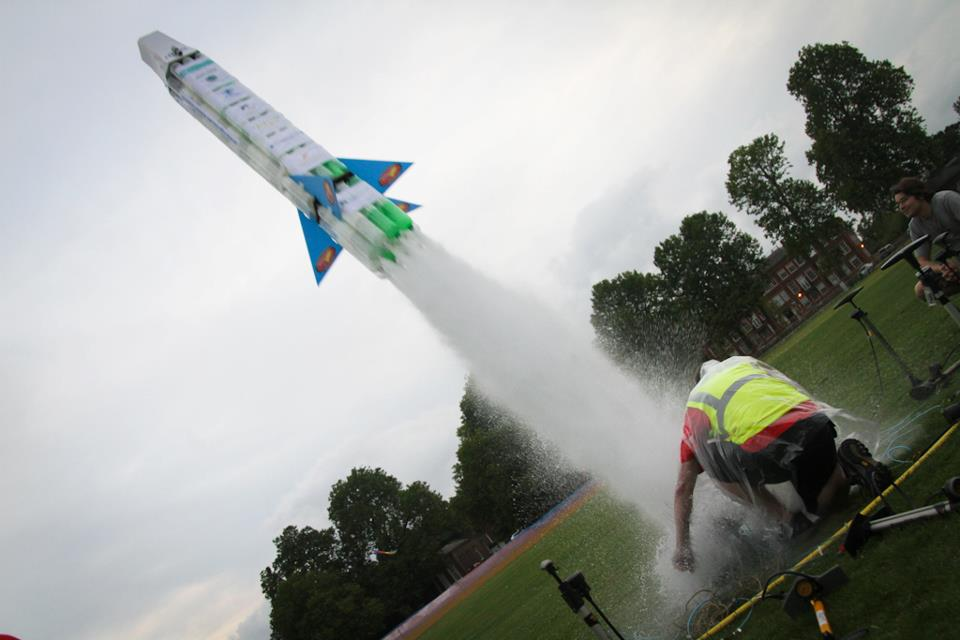
\includegraphics[width=5cm]{cohete4} \vspace{1cm}
	 	\end{center}
	 }
	  \headerbox{MATERIALES}{name=materiales,column=1,row=0,span=2}{
	  	\begin{itemize}
	  \item 2 botellas de dos litros.
	  \item Un tap�n de corcho.
	  \item Una aguja para inflar pelotas.
	  \item Una bomba de aire.
	  \item Un cart�n de leche.
	  \item Un marcador.
	  \item Un c�ter.
	  \item Una pistola de silicona caliente.
	  \item Cinta adhesiva.
	  
	  	\end{itemize}	
	  }
	  \headerbox{PASOS A SEGUIR}{name=pasos,below=materiales,column=1,span=2}{
	  	\begin{enumerate}
	  	\item Cortar con el c�ter el cono de una de las botellas.
	  	
	  	\item Pegar con silicona caliente a la parte inferior de la otra. 
	  	
	  	\item La parte sobrante la vamos a utilizar de soporte, as� que hacemos un agujero por el que despu�s meteremos la manguera de la bomba de aire, m�s o menos en la mitad de �ste.
	  	
	  	\item Lo siguiente que tenemos que hacer son las alas de nuestro cohete. Para ello, trazamos con el marcador una l�nea de esquina a esquina por una de las caras y cortar por aqu� con el c�ter. 
	  	
	  	\item Pegar a los laterales de nuestro cohete las alas con silicona caliente y fijar bien con cinta adhesiva.
	  	
	  	\item Introducir la aguja con fuerza por el tap�n de corcho, de manera que salga por el otro lado. 
	  	
	  	\item Meter la manguera por el agujero que hemos hecho anteriormente en el soporte de lanzamiento, el cual tendr� que estar lleno de arena o piedras para que se quede fijo en el suelo.
	  	
	  	\item Tan s�lo echar unos 400 ml de agua en el cohete casero y dar presi�n con la bomba hasta que salga despedido.
	  	
	  	\end{enumerate}
	  	
	  }
	  
	  \headerbox{OTRAS RECOMENDACIONES}{name=otras,below=pasos,column=1,span=2}{
	  Aparte de lo que hemos comentado de como llevar a cabo un cohete impulsado por agua, tambi�n se pueden hacer otras muchas modificaciones:
	  \begin{itemize}
	  	\item Colocaci�n de varias fases para que se impulse mucho m�s alto.
	  	\item Elaboraci�n de una estructura de lanzamiento mejorada, que permita la compresi�n del gas y mediante una palanca soltar el cohete para aumentar el realismo.
	  	\item Fabricaci�n de un paraca�das para frenar el impacto, con un temporizador que salte en un momento determinado de la ca�da. 
	  	\item Elementos decorativos como pintarle las alas, pintar y elaborar una estructura donde ir� el cohete.
	  \end{itemize} 
	  	
	  	}
	  	
	   \headerbox{PRECAUCIONES}{name=precauciones,below=otras,column=1,span=2}{
	   	Hay que tener en cuenta algunas recomendaciones a la hora de llevar a cabo la construcci�n del cohete:
	   	\begin{itemize}
	   		\item Debido a que sale disparado es conveniente que se utilice protecci�n y que se mantenga una distancia de seguridad.
	   		\item Como se va a meter presi�n en la botella hay que tener precauci�n con que no estalle y que si estalla se est� lo m�s lejos y protegido posible.
	   		\item A la hora de tratar con la silicona y el c�ter hay que tener especialmente cuidado pues son elementos que pueden causar lesiones cut�neas.
	   	\end{itemize}
	   	\vspace{0.1cm}
	   	
	   }

\end{poster}
\end{document}

